\section{Results} \label{sec_res}
In this section, we show two Fourier analysis: one where the $S_n$ order is
varied and one where the aspect ratio is varied. We also compare different
methods to solve MIP: conjugate gradient (CG), conjugate gradient
preconditioned with symmetric Gauss-Seidel (PCG-SGS), conjugate gradient
preconditioned with ML using uncoupled aggregation (PCG-ML-Uncoupled),
conjugate gradient preconditioned with ML using MIS aggregation (PCG-ML-MIS),
and AGMG. The options used for ML can be found in the Appendix.
\subsection{Fourier Analysis}
Analysing Source Iteration accelerated with DSA is often performed thanks to
Fourier analysis \cite{larsen_dsa,consistent_p1}. When a Fourier analysis is
performed, the error is decomposed into different modes and by inspecting the 
damping of the different error modes, the effectiveness of the DSA scheme can 
be studied. The largest damping factor is the spectral radius of the method. 
The smaller
the spectral radius is, the faster the scheme converges. If the spectral
radius is greater than one, the method is unstable. Next, we present two Fourier 
analysis. In the first one, the $S_n$ order is varied whereas in the second one, 
the aspect ratio of the cell is modified.
\subsubsection{$S_n$ order varied}
This Fourier analysis was carried on a square cell, using a
Gauss-Legendre-Chebyshev (GLC) quadrature. The medium is homogeneous, the scattering
ratio $c=0.9999$ and periodic boundary conditions are used. The $x-$axis is the mesh
size in mean free path and the $y-$axis is the spectral radius. There are four
curves corresponding to different $S_n$ order: $S_2$, $S_4$, $S_8$ and
$S_{16}$.
\begin{figure}[H]
\centering
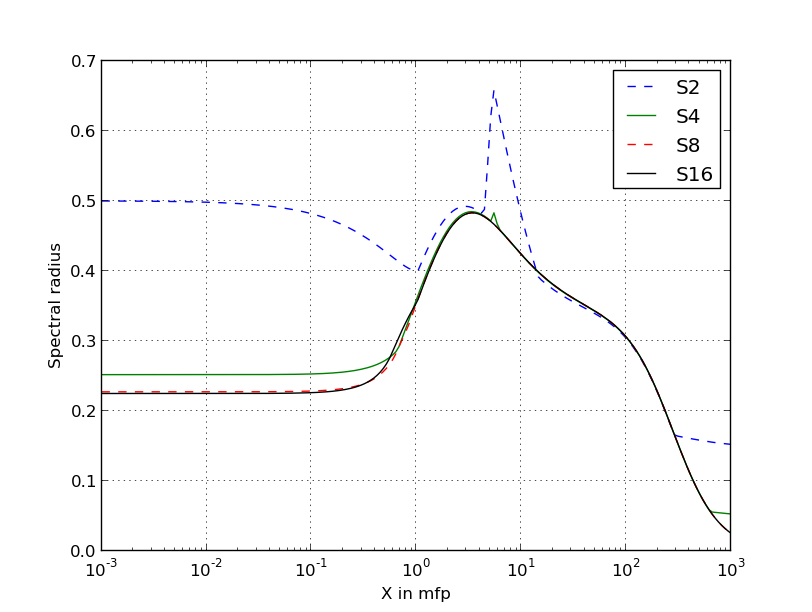
\includegraphics[width=0.5\textwidth]{sn_order_9999}
\caption{Fourier analysis as a function of the mesh optical thickness,
homogeneous infinite medium case.}
\end{figure}
MIP is stable for every cell size. The spectral radius is always less than
0.5, except for $S_2$ where it is about 0.7.
\subsubsection{Aspect ratio varied}
For this Fourier analysis, we use a $S_{16}$ GLC quadrature, a homogeneous
medium, $c=0.9999$ and periodic boundary conditions. The $x-$axis is the mesh
size in mean free path in the $x$ direction and the $y-$axis is the spectral
radius. There are five curves corresponding to five different aspect ratio:
$\frac{Y}{X}=\frac{1}{16}$, $\frac{Y}{X}=\frac{1}{4}$, $\frac{Y}{X}=1$,
$\frac{Y}{X}=4$ and $\frac{Y}{X}=16$. 
\begin{figure}[H]
\centering
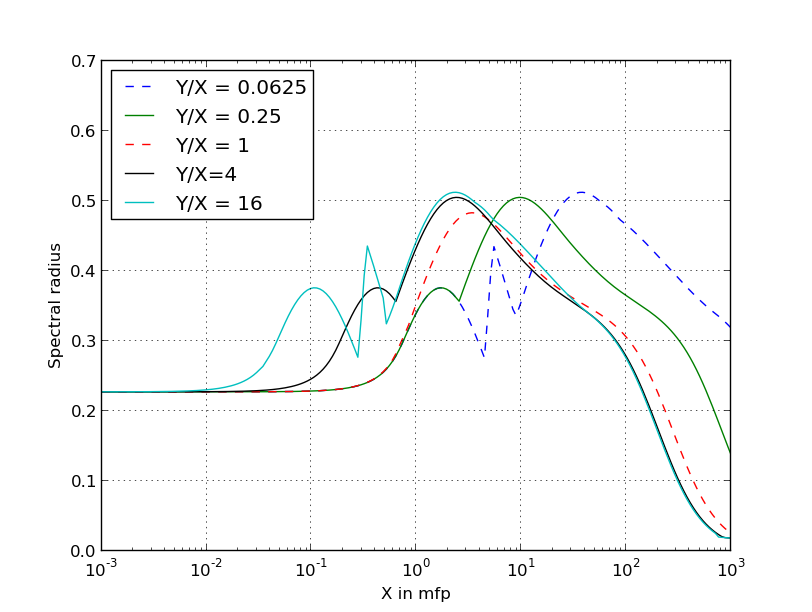
\includegraphics[width=0.5\textwidth]{aspect_ratio_9999}
\caption{Fourier analysis as a function of the mesh optical thickness,
homogeneous infinite medium case for different aspect ratios.}
\end{figure}
MIP is stable for every the aspect ratio and the maximum of the spectral radius
is at about 0.5

\subsection{Homogeneous medium}
Next we compare different solvers for MIP on a homogeneous medium, 10cm $\times$
10cm, $\Sigma_t=1$cm$^{-1}$ and $\Sigma_s=0.99$cm$^{-1}$ with vacuum boundary 
conditions and a source of intensity 1cm$^{-3}$s$^{-1}$. We use a $S_8$
Gauss-Legendre-Chebyshev quadrature, a Source Iteration solver with relative
tolerance of $10^{-8}$ and a relative tolerance for MIP of $10^{-10}$.
\subsubsection{Quadrilateral cells}
In this example, the mesh is composed of 9990 quadrilateral cells that corresponds 
to 39960 degrees of freedom. The solution is:
\begin{figure}[H]
\centering
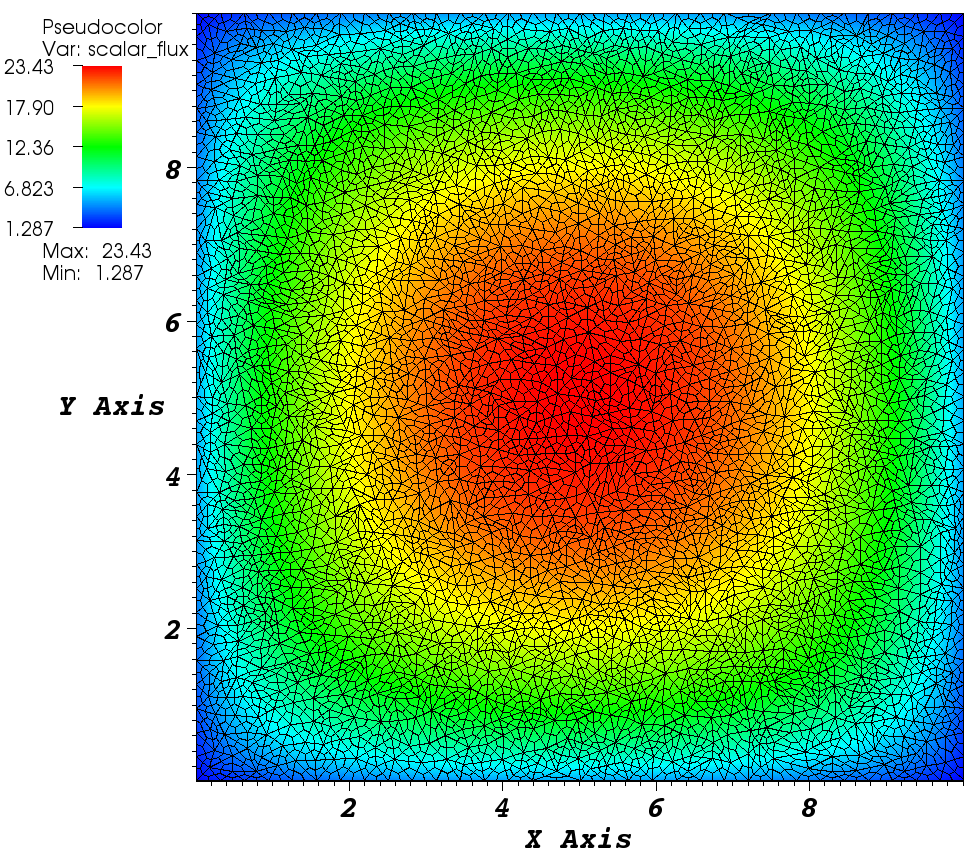
\includegraphics[width=0.6\textwidth]{homog_quad_crop}
\caption{Quadrilateral cells.}
\end{figure}
In the next table, the different solvers are compared:
\begin{table}[H]
\begin{center}
\begin{tabular}{|c|c|c|c|c|c|c|}
\hline
 & No-DSA & CG & PCG-SGS & PCG-ML-Uncoupled & PCG-ML-MIS & AGMG\\
\hline
SI iterations & 268 & 27 & 27 & 27 & 27 & 27 \\
Precond init (s) & NA & NA & 0.0142572 & 0.381872 & 1.21095 & 0.068\\
MIP calculation (s) & NA & 138.379 & 177.556 & 46.1957 & 44.7837 & 6.9311\\
CG iterations & NA & 35419 & 11414 & 729 & 702 & 674\\
Total calculation (s) & 309.395 & 172.181 & 211.933 & 80.1548 & 80.0387 &
40.827\\
\hline
\end{tabular}
\caption{Comparison of preconditioners with quadrilateral cells.}
\end{center}
\end{table}
In this Table, SI iterations is the number iteration of Source Iteration
needed to solve the problem, Precond init is the time in seconds needed to
initialize the preconditioner used by CG, MIP calculation is the total time in
seconds spent solving DSA during the calculation, CG iterations is the total number 
of CG iterations used to solve MIP, and Total calculation is the time in
seconds needed to solve the problem.

Using MIP decreases significantly the number of SI iterations and the
calculation time as expected. Using PCG-SGS decreases by a factor three the 
number of CG iterations compared to CG but the time needed to solve MIP is
greater. With ML, the number of CG iterations is reduced by a factor 50 and 
the MIP calculation time is divided by three compared to CG. AGMG is by far 
the most efficient solver, the number of CG iteration is slightly lower 
than PCG-ML but the MIP calculation is 20 times faster than CG.

\subsubsection{Polygonal cells}
In this problem, the mesh is composed of 13654 triangles, 250 quadrilaterals,
1400 pentagons, 1306 hexagons, 228 heptagons, and 6 octagons, for a total of
16844 cells and 58442 degrees of freedoms. This example will allow us to test
MIP and the different preconditioners on a mesh composed of different types of
cell. The solution and the mesh are:
\begin{figure}[H]
\centering
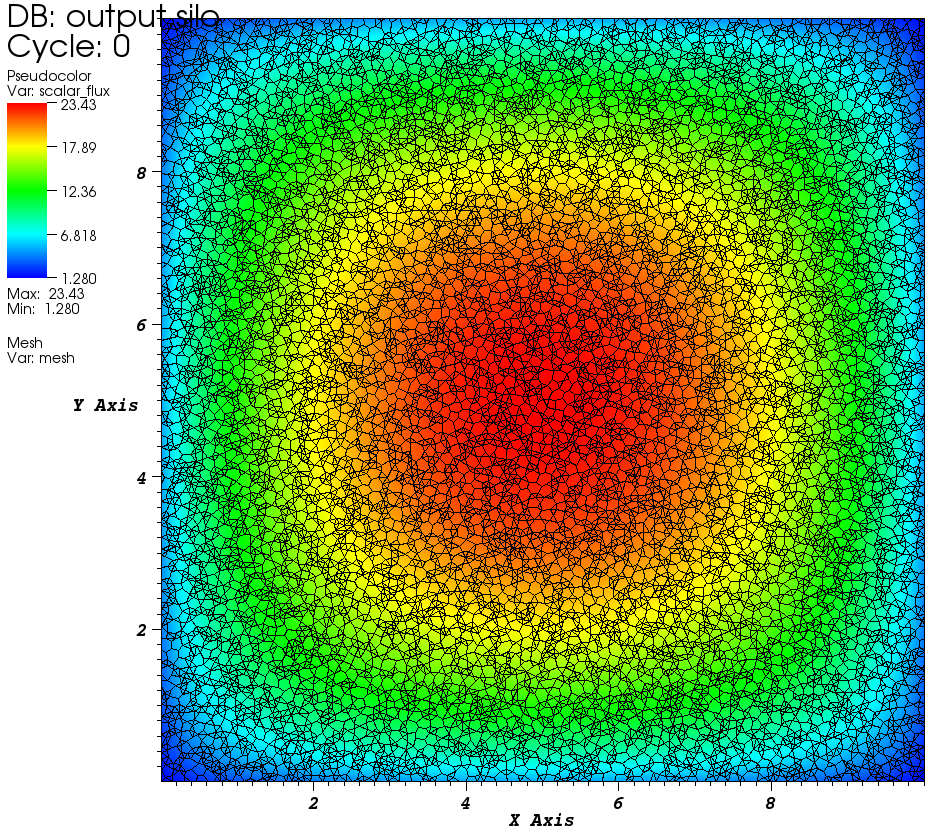
\includegraphics[width=0.6\textwidth]{homog_poly_crop}
\caption{Polygonal cells.}
\end{figure}
The different solvers are compared in the next Table:
\begin{table}[H]
\begin{center}
\begin{tabular}{|c|c|c|c|c|c|c|}
\hline
 & No-DSA & CG & PCG-SGS & PCG-ML-Uncoupled & PCG-ML-MIS & AGMG\\
\hline
SI iterations & 268 & 27 & 27 & 27 & 27 & 27\\
Precond init (s) & NA & NA & 0.0201421 & 0.482845 & 2.09054 & 0.097\\
MIP calculation (s) & NA & 210.128 & 303.423 & 78.0993 & 71.4493 & 11.0419\\
CG iterations & NA & 36352 & 13370 & 840 & 784 & 674\\
Total calculation (s) & 458.132 & 265.026 & 358.745 & 134.434 & 128.731 &
66.0207\\
\hline
\end{tabular}
\caption{Comparison of preconditioners with polygonal cells.}
\end{center}
\end{table}
We see that using different types of cells in the same mesh does not affect
the performance of MIP or of the preconditioners. 

\subsection{Heterogeneous medium}
In this example, we use a heterogeneous medium composed of 184 triangles, 3720
quadrilaterals and 2791 regular hexagons of side 0.05$cm$ for a total of 6695 
cells and 32178 degrees of freedom. The domain is 5.28275$cm$ by 4.6$cm$. 
Reflective boundary conditions are used. The quadrature is a $S_{16}$ 
Gauss-Legendre-Chebyshev quadrature. The SI solver has a relative tolerance of 
$10^{-8}$ and the relative tolerance for MIP is $10^{-10}$. The domain is 
composed of three zones:
\begin{figure}[H]
\centering
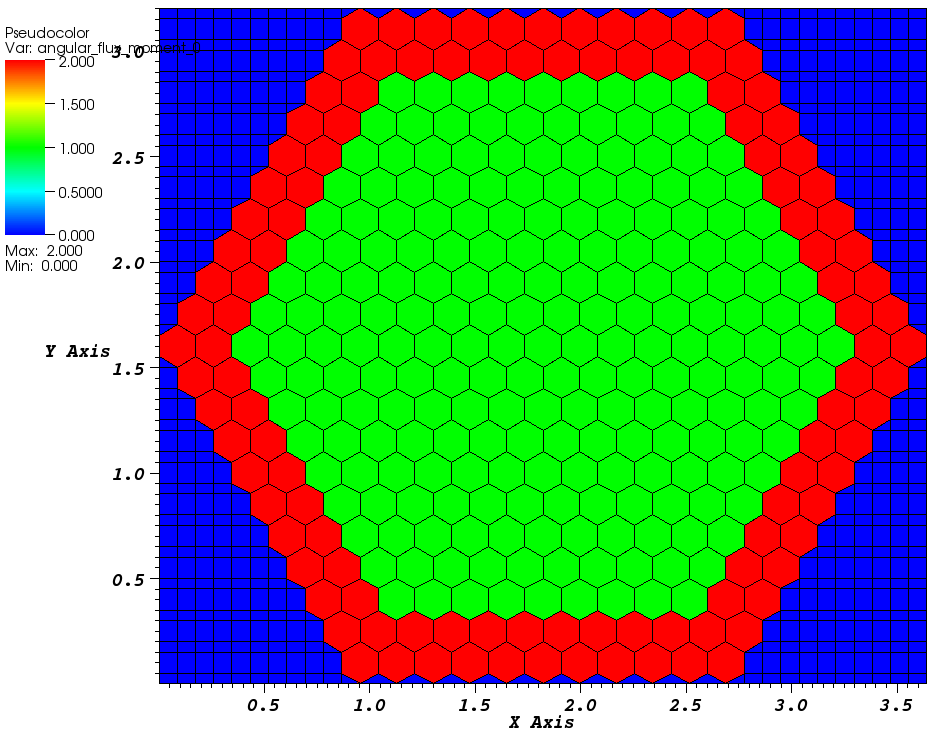
\includegraphics[width=0.4\textwidth]{source_crop}
\caption{Zones of the domain.}
\end{figure}
The properties of the different zones are:
\begin{description}
\item[Green zone:] $\Sigma_t =1$cm$^{-1}$, $\Sigma_s = 0.9$cm$^{-1}$, source$ =
1$cm$^{-3}$s$^{-1}$
\item[Red zone:] $\Sigma_t = 1.5$cm$^{-1}$, $\Sigma_s = 1.44$cm$^{-1}$, no source
\item[Blue zone:] $\Sigma_t = 1$cm$^{-1}$, $\Sigma_s = 0.3$cm$^{-1}$, no source
\end{description}
The scalar flux for this problem is:
\begin{figure}[H]
\centering
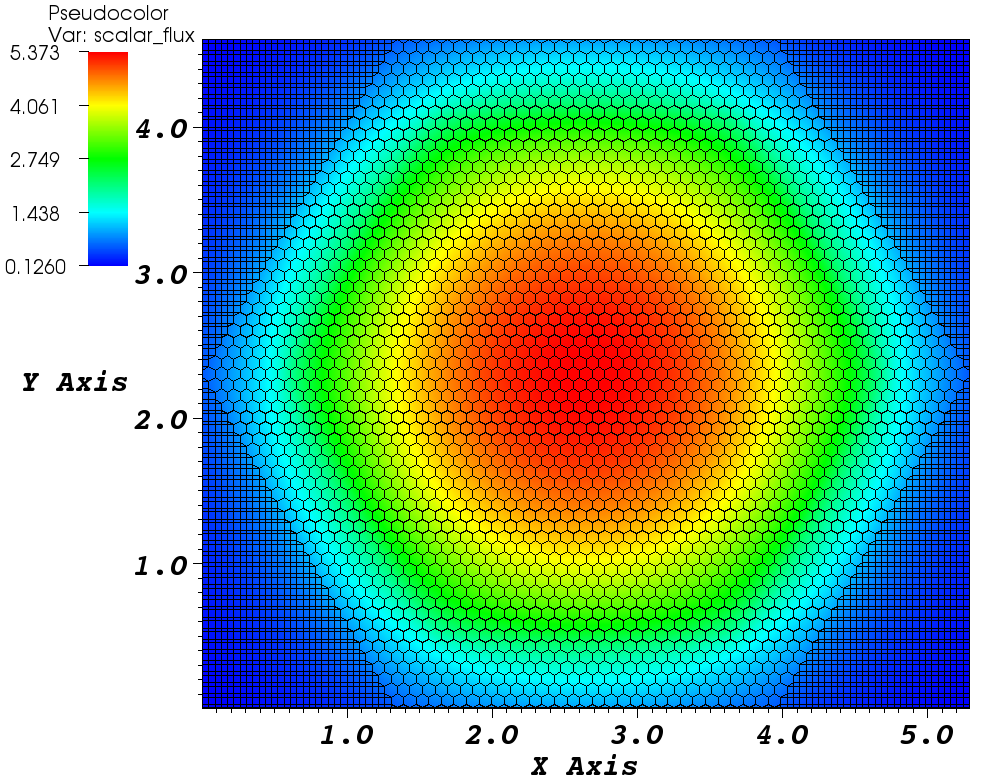
\includegraphics[width=0.6\textwidth]{heterog_hex_crop}
\caption{Hexagonal cells.}
\end{figure}
The different solvers are compared in the next Table:
\begin{table}[H]
\begin{center}
\begin{tabular}{|c|c|c|c|c|c|c|}
\hline
 & No-DSA & CG & PCG-SGS & PCG-ML-Uncoupled & PCG-ML-MIS & AGMG\\
\hline
        SI iterations & 111     & 19      & 19        & 19      & 19      & 19 \\
     Precond init (s) & NA      & NA      & 0.0159521 & 0.49212 & 1.31818 &
0.108 \\
  MIP calculation (s) & NA      & 51.7628 & 82.5123   & 30.987  & 29.7762 &
2.64274 \\
        CG iterations & NA      & 10216   & 4481      & 423     & 402     & 260 \\
Total calculation (s) & 379.175 & 121.798 & 147.094   & 94.7139 & 94.8013 &
65.5546 \\
\hline
\end{tabular}
\caption{Comparison of preconditioners with heterogeneous medium.}
\end{center}
\end{table}
We can see that the comments that were done for the homogeneous tests are
still valid. MIP is effective even with heterogeneous medium and the AGMG is
still the fastest solver.
